\documentclass[a4paper, 10pt, titlepage, twoside]{article}

\usepackage[T2A]{fontenc}
\usepackage[utf8]{inputenc}
\usepackage[russian,english]{babel}
\usepackage{graphicx}
\usepackage{svg}

\usepackage{hyperref}
\hypersetup{
    colorlinks=false,
    pdfborder={0 0 0},
}

\usepackage{fullpage}

\begin{document}
\title{How to Structure a LaTeX Document}
\begin{titlepage}
  \begin{center}
    \vspace{10pt}
    \includesvg[height=120pt]{lambda}
    \\
    \vspace{120pt}
    \Huge{Методическое пособие по языку Common Lisp.}
    \end{center}
\end{titlepage}

\section{Lispbox}
Lispbox --- небольшая, но функциональная среда разработки для языка Common Lisp. Она представляет собой текстовый редактор Emacs связанный с лисп-системой Clozure Common Lisp через расширение Slime (\textbf{S}uperior \textbf{L}isp \textbf{I}nteraction \textbf{M}ode for \textbf{E}macs). Также в lispbox входит настроенная для работы система управления пакетами quicklisp. Из-за почтенного возраста ключевого компонента системы --- редактора Emacs, которому в следующем году исполнится 38 лет, некоторые особенности управления могут оказаться странными или запутывающими, однако на практике они оказываются довольно удобными и впоследствии вызывают сильное привыкание.
\subsection{Установка}
Домашняя страница проекта: \url{http://common-lisp.net/project/lispbox/}. Lispbox распространяется в виде zip-архива и не требует установки. Просто скачайте архив и распакуйте его в удобное вам место, например C:\textbackslash{}Users
\textbackslash{}Alex\textbackslash{}Lisp\textbackslash{}lispbox. К сожалению, у lispbox иногда возникают проблемы с кириллическими путями, поэтому может понадобиться распаковка в место, путь к которому содержит только латинские символы.
По-умолчанию lispbox не поддерживает нелатинские символы, но их поддержку несложно добавить. Для это нужно выполнить следующие действия:
\begin{itemize}
\item В директории, в которую вы распаковали lispbox, найдите файл lispbox.bat и замените в нем строку 
  \footnotesize
  \begin{verbatim} set TO_EVAL="(progn (load \"lispbox\") (slime))" \end{verbatim}
  \normalsize
  на строку
  \footnotesize
  \begin{verbatim} set TO_EVAL="(progn (setq slime-net-coding-system 'utf-8-unix)(load \"lispbox\") (slime))" \end{verbatim}
  \normalsize
\item В подкаталоге slime-* в файле swank-loader.lisp в самое начало файла добавьте строку
  \footnotesize
  \begin{verbatim} (setf CCL:*DEFAULT-EXTERNAL-FORMAT* :utf-8) \end{verbatim}
  \normalsize
\end{itemize}
Теперь lispbox поддерживает русский язык (как впрочем и другие языки с нелатинской письменностью).

Для запуска среды дважды щелкните по файлу \verb lispbox.bat . Если всё прошло успешно, сначала вы увидите лог процесса запуска системы, а потом вас поприветствует следующее окно:
\begin{center}
  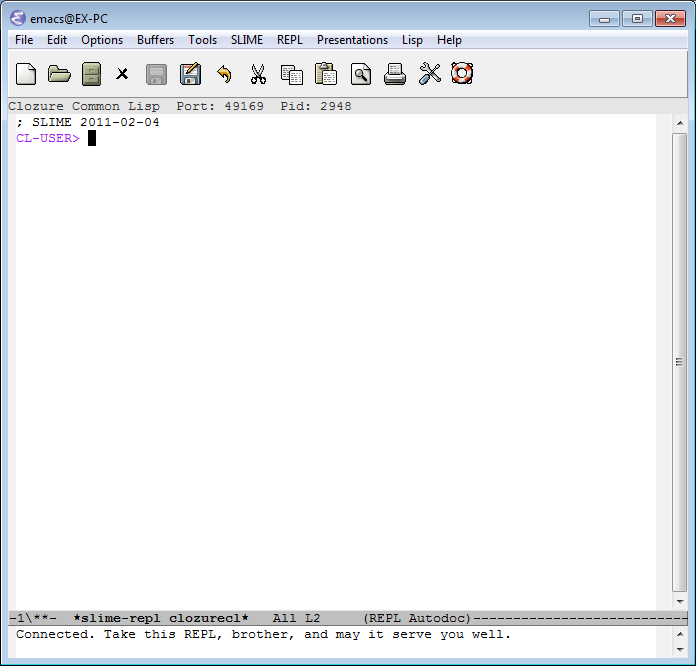
\includegraphics[scale=.6]{lispbox_started}\\
  \small{\textit{Запущенный lispbox}}
\end{center}
\subsection{Работа в lispbox}
Emacs --- основа выбранной нами IDE --- крайне гибкий и мощный инструмент, однако, довольно требовательный к пользователю. Безграничный потенциал Emacs и его отличия от традиционных текстовых редакторов породили множество легенд о сложности в освоении и использовании. Но это совсем не так. Совершим небольшой экскурс по основным понятиям и командам Emacs.
\subsubsection{Буфер}
\item{Буфером} называется во-первых любой открытый файл, а во-вторых вообще любое пространство, в которое вводится или выводится информация. Название буфера пишется внизу слева. Все буферы перечислены в верхнем меню Buffer. Как видно, после старта lispbox по умолчанию открыты буферы под названиями *scratch*, *Messages*, *slime-events*, *slime-repl clozurecl* и *inferior-lisp*. Первые два являются стандартными буферами Emacs, следующие два --- служебные буферы Slime, и наконец последний --- интерпретатор, открытый сейчас перед нами. Обратите внимание на название буфера, написанное слева внизу.
\begin{center}
  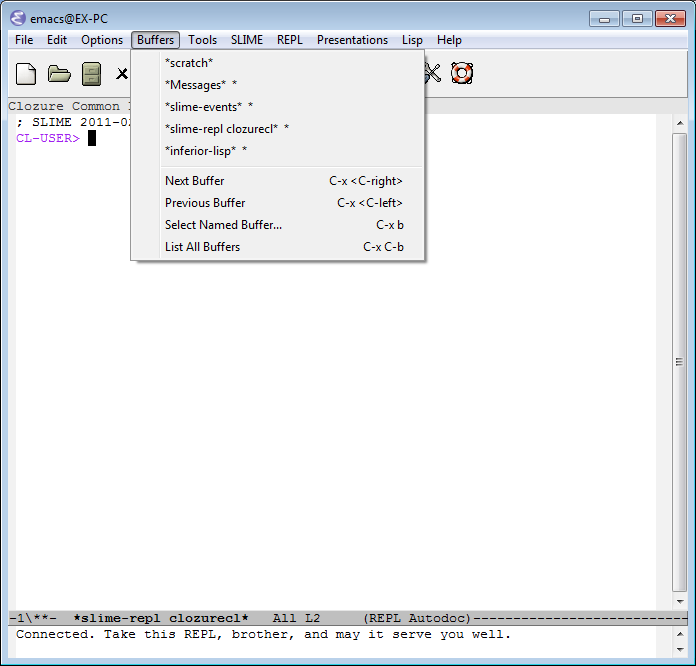
\includegraphics[scale=.6]{lispbox_buffers}\\
  \small{\textit{Буферы по умолчанию}}
\end{center}
\subsubsection{Горячие клавиши}
На рисунке выше внизу выпадающего меню рядом с командами находятся сочетания клавиш, также иногда называемые аккрдами, назначенные на эти команды.
Такие сочетания используются в Emacs повсеместно, и после некоторого привыкания очень сильно облегчают работу. Однако, конвенция, принятая в Emacs, довольно сильно отличается от всех остальны программ, и требует пояснения. 
Рассмотрим, к примеру, команду Next-buffer. Как видно из скиншота выше, этой команде назначено сочетание C-x <C-left>. Буквой С в Emacs обозначается нажатие на клавишу Control. Запись C-x обозначает всего-навсего сочетание Control-x. Последовательность C-x <C-left> же означает, что сначала нужно набрать Control-x, а потом Control-<стрелка влево>. Сделать это можно и не отпуская клавишу Control, то есть зажать Control, потом нажать и отпустить x, а потом нажать стрелку влево.
Если префикс С- не указан, значит нажатие на Control не нужно. То есть С-х b есть комбинация Control-x, за которой следует нажатие на кнопку b уже при отпущенной клавише Control. Основные команды работы с буферами, многие из которых также доступны через меню ``File'' и ``Buffers'', перечислены ниже:
\begin{itemize}
\item C-x C-f открывает файл с с введенным именем. Если файл есть, открывает для редактированияб если нет --- создает новый
\item C-x b <имя буфера> переключается на буфер с введенным именем. Если такого буфера нет, то он будет создан
\item C-x C-b создает новое \textit{окно}, в которое выводит список существует буферов
\item C-x k закрывает буфер, в котором находится курсор. Если буфер остался один, закрыть его нельзя. Если вы попытаетесь закрыть буфер, открытый на файле, и имеющий несохраненные данные, Emacs попросит подтверждения выполнения
\item C-x C-s сохраняет содержимое буфера в текстовый файл
\end{itemize}
\subsubsection{Окна}
Emacs использует термин ``окно'' в несколько отличном от привычного смысле. Окно в том же смысле, в котором его используем мы, то есть в смысле отдельного окна опрерационной системы, в Emacs называется \textit{фреймом}. Окном же называется область, в которой отображается ровно один буфер. Новые окна можно получить, деля существующие по горизонтали или по вертикали. Две команды для работы с окнами можно найти в меню ``File''. Некоторые команды для работы с окнами:
\begin{itemize}
\item C-x 2 делит окно по горизонтали
\item C-x 3 делит окно по вертикали
\item C-x 0 закрывает окно, в котором находится курсор, сливая его с ближайшим соседним окном. Как и в случае с буфером, закрыть последнее открытое окно нельзя. Обратите внимание, что буфер, отображавшийся в окне, никуда не пропадает, и вернуться к нему можно при помощи команды C-x b
\item C-x 1 разворачивает выбранное окно на весь фрейм. Также это можно трактовать как закрытие всех окон, кроме выбранного
\item
\item
\end{itemize}
\section{Интерпретатор}
Итак, среда запущена и готова к работе. Вы видите перед собой приглашение, гласящее \verb Cl-USER> . Такой режим работы Лиспа называется REPL --- Read-Eval-Print Loop, также известный как интерактивный режим или \textit{toplevel}. Суть его заключается в том, что пользователь напрямую общается с лисп-системой, производя вычисления и получая ответы в реальном времени. Этот режим, впервые появившийся в Лиспе, отличает его от статических, компилируемых языков типа Фортрана, С или Java, и присутствует практически во всех динамических языках, например Ruby, Python и Perl. Несмотря на то, что этот режим присущ интерпретируемым языкам, почти все современные реализации Common Lisp являются компилируемыми, и Clozure CL в этом плане не исключение.

Числа и строки являются самыми простыми выражениями, доступными программисту, и вычисляются сами в себя. Поприветствуйте lispbox, введя в строке приглашения что-нибудь вроде ``Привет, Лисп!'', и нажав Enter. Строка, введенная вами, выведется на экран, а после неё снова появится строка приглашения. То же самое произойдет, если вводить числа, простые и десятичные дроби, а также некоторые другие выражения:
\begin{center}
  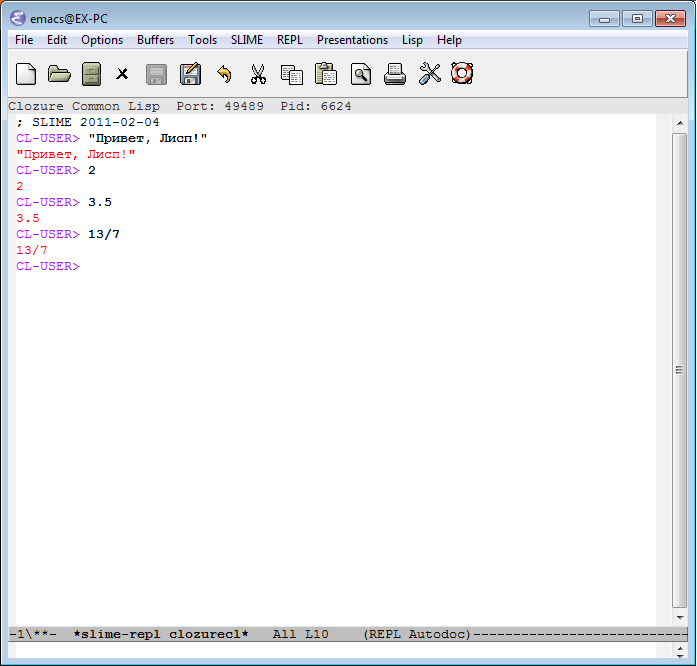
\includegraphics[scale=.7]{lispbox_toplevel}\\
  \small{\textit{Простейшие выражения}}
\end{center}
Теперь рассмотрим некоторые более сложные примеры команд. Например, если мы хотим сложить два числа 1 и 2, следует ввести (+ 1 2). Как несложно заметить, такая запись несколько отличается от общепринятой в математике, да и в других языках программирования. Поначалу это кажется непривычным, однако такой подход на самом деле более универсален: для записи сложения трех чисел обычная запись требует использования уже двух знаков ``+'', в то время как в префиксной нотации, принятой в Лиспе, сложение трех чисел будет выглядеть так: (+ 1 2 3). Как и для четырех и более.
\end{document}
        

